%%
\clearpage
\newpage
\section{The cal\_SLIT recipe}
\label{ch:the_recipes:cal_SLIT_spirou}
%%
%%%%%%%%%%%%%%%%%%%%%%%%%%%%%%%%%%%%%%%%%%%%%%%%%%%%%%%%

Fabry-Perot exposures in which the three fibres are simultaneously fed by light from the Fabry-Perot filter. Each exposure is used to build the slit orientation. Finds the tilt of the orders. \\

% -------------------------------------------------------
\subsection{The inputs}
% -------------------------------------------------------
The input of {\calSLIT} is as follows:
\begin{cmdbox}
cal_SLIT_spirou.py night_repository filenames
\end{cmdbox}
\noindent for example:
\begin{cmdbox}
cal_SLIT_spirou.py 20170710 fp_fp02a203.fits fp_fp03a203.fits fp_fp04a203.fits
\end{cmdbox}
\noindent or
\begin{pythonbox}
import cal_SLIT_spirou
night_repository = '20170710'
filenames = ['fp_fp02a203.fits', 'fp_fp03a203.fits', 'fp_fp04a203.fits']
cal_SLIT_spirou.main(night_repository, files=filenames)
\end{pythonbox}

\noindent where `night\_repository' defines \argnightname and `filenames' define the list of files in \argfilenames. All files in filenames must be valid python strings separated by a space (command line) or in a line (python) and must have the following prefixes:
\begin{itemize}
	\item fp\_fp
\end{itemize}

% -------------------------------------------------------
\subsection{The outputs}
% -------------------------------------------------------
The outputs of \calSLIT are as follows:

\begin{itemize}
\item \definevariable{text:tiltfits}{tiltfits} in form:
\begin{tcustomdir}
\{\reduceddir\}/\{date prefix\}\_\{file\}\_tilt.fits
\end{tcustomdir}

\end{itemize}

\noindent where `date prefix' is constructed from \argnightname and the file name is the first file in \argfilenames.

\noindent for example for \reduceddir\lstinline[style=pythoninline]|='/drs/data/reduced/20170710'| and \argfilenames\lstinline[style=pythoninline]|=['fp_fp02a203.fits', 'fp_fp03a203.fits', 'fp_fp04a203.fits']| the output files would be:
\begin{tcustomdir}
\begin{itemize}
\item \path{/drs/data/reduced/20170710/20170710_fp_fp02a203_tilt.fits}
\end{itemize}
\end{tcustomdir}

% -------------------------------------------------------
\subsection{Summary of procedure}
% -------------------------------------------------------
\begin{enumerate}
\item adds all fp\_fp files together
\item corrects for dark
\item resizes the image
\item extracts the orders (no weight no tilt)
\item works out the tilt for each order using the location and width
\item saves the tilt to file
\item should do some quality control
\item  updates calibDB with key ``TILT''
\end{enumerate}


% -------------------------------------------------------
\subsection{Quality Control}
% -------------------------------------------------------

There are currently two quality control checks for \calSLIT
\begin{itemize}

\item Abnormal RMS of SLIT angle if:
\begin{thighlight}
\begin{equation}
\text{RMS}_\text{tilt} > \text{\definevariable{text:qc_slit_rms}{qc\_slit\_rms}}
\end{equation}
\end{thighlight}

\item Abnormal SLIT angle if:
\begin{thighlight}
\begin{equation}
\text{max}(\text{tilt}) > \text{\definevariable{text:c_slit_max}{qc\_slit\_max}}
\end{equation}
or
\begin{equation}
\text{min}(\text{tilt}) < \text{\definevariable{text:c_slit_min}{qc\_slit\_min}}
\end{equation}
\end{thighlight}

\end{itemize}

\noindent If none of these quality control criteria are valid then the output file is passed into the \calibdb with key `TILT'. \\

\noindent For example the following lines are added to the \calibdb for 
\argnightname{\lstinline[style=pythoninline]| = "20170710" |} and \argfilenames{\lstinline[style=pythoninline]| = ['fp_fp02a203.fits', 'fp_fp03a203.fits', 'fp_fp04a203.fits'] |}. \\

\begin{textbox}[title={In calibration database file}]
TILT 20170710 20170710_fp_fp02a203_tilt.fits 2017-07-10-13:25:15.590000 1499693115.59
\end{textbox}


% -------------------------------------------------------
\subsection{Example working run}
% -------------------------------------------------------

An example run where everything worked is below:
\begin{cmdbox}
cal_SLIT_spirou.py 20170710 fp_fp02a203.fits fp_fp03a203.fits fp_fp04a203.fits
\end{cmdbox}
\begin{cmdboxprintspecial}[fontupper=\tiny, fontlower=\tiny]
@gHH:MM:SS.S -   || *****************************************@g
@gHH:MM:SS.S -   || * SPIROU \@(#) Geneva Observatory (VERSION)@g
@gHH:MM:SS.S -   || *****************************************@g
@gHH:MM:SS.S -   ||(dir_data_raw)      DRS_DATA_RAW=/drs/data/raw@g
@gHH:MM:SS.S -   ||(dir_data_reduc)    DRS_DATA_REDUC=/drs/data/reduced@g
@gHH:MM:SS.S -   ||(dir_calib_db)      DRS_CALIB_DB=/drs/data/calibDB@g
@gHH:MM:SS.S -   ||(dir_data_msg)      DRS_DATA_MSG=/drs/data/msg@g
@gHH:MM:SS.S -   ||(print_level)       PRINT_LEVEL=all         %(error/warning/info/all)@g
@gHH:MM:SS.S -   ||(log_level)         LOG_LEVEL=all         %(error/warning/info/all)@g
@gHH:MM:SS.S -   ||(plot_graph)        DRS_PLOT=1            %(def/undef/trigger)@g
@gHH:MM:SS.S -   ||(used_date)         DRS_USED_DATE=undefined@g
@gHH:MM:SS.S -   ||(working_dir)       DRS_DATA_WORKING=/drs/data/tmp@g
@gHH:MM:SS.S -   ||                    DRS_INTERACTIVE is not set, running on-line mode@g
@gHH:MM:SS.S -   ||                    DRS_DEBUG is set, debug mode level:1@g
@gHH:MM:SS.S -   |cal_SLIT_spirou:2a203+[...]|Now running : cal_SLIT_spirou on file(s): fp_fp02a203.fits, fp_fp03a203.fits, fp_fp04a203.fits@g
@gHH:MM:SS.S -   |cal_SLIT_spirou:2a203+[...]|On directory /drs/data/raw/20170710@g
@gHH:MM:SS.S -   |cal_SLIT_spirou:2a203+[...]|ICDP_NAME loaded from: /scratch/Projects/spirou_py3/spirou_py3/INTROOT/config/constants_SPIROU.py@g
@gHH:MM:SS.S - * |cal_SLIT_spirou:2a203+[...]|Correct type of image for slit (f or p or _ or f or p)@g
@gHH:MM:SS.S -   |cal_SLIT_spirou:2a203+[...]|Calibration file: 20170710_flat_flat02f10_badpixel.fits already exists - not copied@g
...
@gHH:MM:SS.S -   |cal_SLIT_spirou:2a203+[...]|Calibration file: spirou_wave_ini3.fits already exists - not copied@g
@gHH:MM:SS.S -   |cal_SLIT_spirou:2a203+[...]|Calibration file: 2017-10-11_21-32-17_hcone_hcone02c406_wave_AB.fits already exists - not copied@g
@gHH:MM:SS.S -   |cal_SLIT_spirou:2a203+[...]|Calibration file: spirou_wave_ini3.fits already exists - not copied@g
@gHH:MM:SS.S -   |cal_SLIT_spirou:2a203+[...]|Calibration file: 2017-10-11_21-32-17_hcone_hcone02c406_wave_C.fits already exists - not copied@g
@gHH:MM:SS.S - * |cal_SLIT_spirou:2a203+[...]|Now processing Image TYPE UNKNOWN with cal_SLIT_spirou recipe@g
@gHH:MM:SS.S -   |cal_SLIT_spirou:2a203+[...]|Reading Image /drs/data/raw/20170710/fp_fp02a203.fits@g
@gHH:MM:SS.S -   |cal_SLIT_spirou:2a203+[...]|Image 2048 x 2048 loaded@g
@gHH:MM:SS.S - * |cal_SLIT_spirou:2a203+[...]|Adding 2 frame(s)@g
@gHH:MM:SS.S -   |cal_SLIT_spirou:2a203+[...]|Reading File: /drs/data/raw/20170710/fp_fp03a203.fits@g
@gHH:MM:SS.S -   |cal_SLIT_spirou:2a203+[...]|Reading File: /drs/data/raw/20170710/fp_fp04a203.fits@g
@gHH:MM:SS.S -   |cal_SLIT_spirou:2a203+[...]|Doing Dark Correction using /drs/data/calibDB/20170710_dark_dark02d406.fits@g
@gHH:MM:SS.S -   |cal_SLIT_spirou:2a203+[...]|Image format changed to 1930x2035@g
@gHH:MM:SS.S - * |cal_SLIT_spirou:2a203+[...]|Nb dead pixels = 611716 / 15.58 %@g
@gHH:MM:SS.S -   |cal_SLIT_spirou:2a203+[...]|Reading localization parameters of Fiber AB@g
@gHH:MM:SS.S -   |cal_SLIT_spirou:2a203+[...]|Order 0.0: Tilt = 4.70 on pixel 37.0 = -7.23 deg@g
@gHH:MM:SS.S -   |cal_SLIT_spirou:2a203+[...]|Order 1.0: Tilt = 4.60 on pixel 37.4 = -7.02 deg@g
@gHH:MM:SS.S -   |cal_SLIT_spirou:2a203+[...]|Order 2.0: Tilt = 4.50 on pixel 36.8 = -6.97 deg@g
@gHH:MM:SS.S -   |cal_SLIT_spirou:2a203+[...]|Order 3.0: Tilt = 4.30 on pixel 36.3 = -6.75 deg@g
...
@gHH:MM:SS.S -   |cal_SLIT_spirou:2a203+[...]|Order 32.0: Tilt = 1.40 on pixel 33.3 = -2.41 deg@g
@gHH:MM:SS.S -   |cal_SLIT_spirou:2a203+[...]|Order 33.0: Tilt = 1.10 on pixel 32.3 = -1.95 deg@g
@gHH:MM:SS.S -   |cal_SLIT_spirou:2a203+[...]|Order 34.0: Tilt = 1.00 on pixel 32.1 = -1.79 deg@g
@gHH:MM:SS.S -   |cal_SLIT_spirou:2a203+[...]|Order 35.0: Tilt = 0.30 on pixel 17.1 = -1.01 deg@g
@gHH:MM:SS.S - * |cal_SLIT_spirou:2a203+[...]AB|Tilt dispersion = 0.091 deg@g
@gHH:MM:SS.S -   |cal_SLIT_spirou:2a203+[...]|Saving tilt  information in file: 20170710_fp_fp02a203_tilt.fits@g
@yHH:MM:SS.S - \@ |python warning Line 980  warning reads: Card is too long, comment will be truncated.|@y
@gHH:MM:SS.S - * |cal_SLIT_spirou:2a203+[...]|QUALITY CONTROL SUCCESSFUL - Well Done -@g
@gHH:MM:SS.S - * |cal_SLIT_spirou:2a203+[...]|Updating Calib Data Base with TILT@g
@gHH:MM:SS.S - * |cal_SLIT_spirou:2a203+[...]|Recipe cal_SLIT_spirou has been successfully completed@gHHMSSS
\end{cmdboxprintspecial}

% -------------------------------------------------------
\newpage
\subsection{Interactive mode}
% -------------------------------------------------------

\noindent In interactive mode three figures will also appear (see Figure \ref{figure:cal_SLIT_spirou}).

\begin{figure}

\begin{center}
\begin{minipage}{.495\textwidth}
\begin{center}
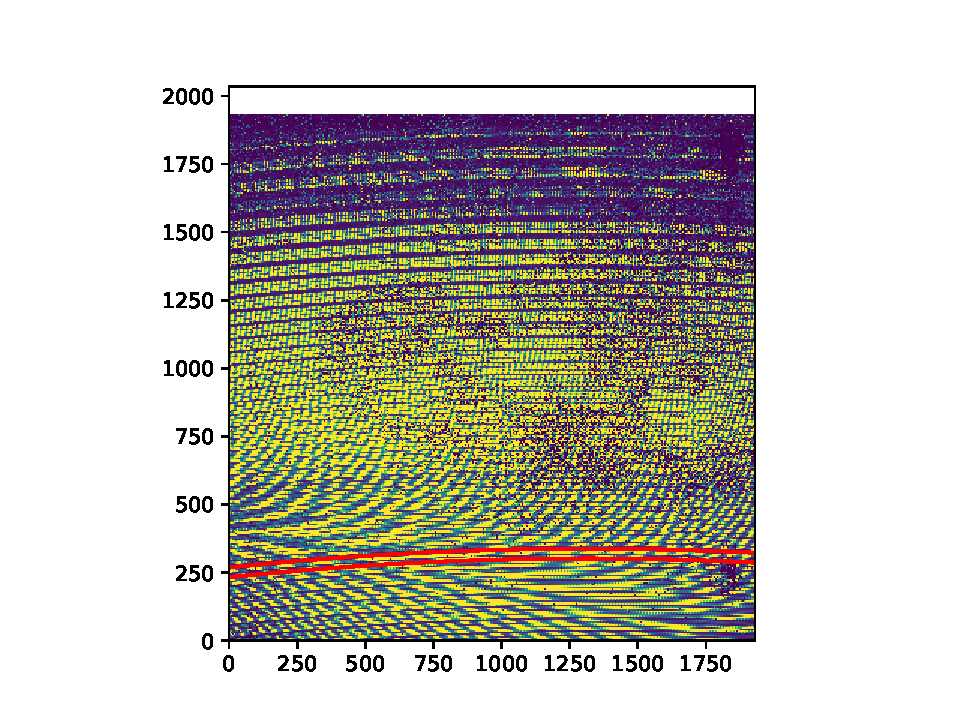
\includegraphics[width=\textwidth]{Figures/cal_SLIT_spirou_1a.pdf}
a
\end{center}
\end{minipage}%
\begin{minipage}{.495\textwidth}
\begin{center}
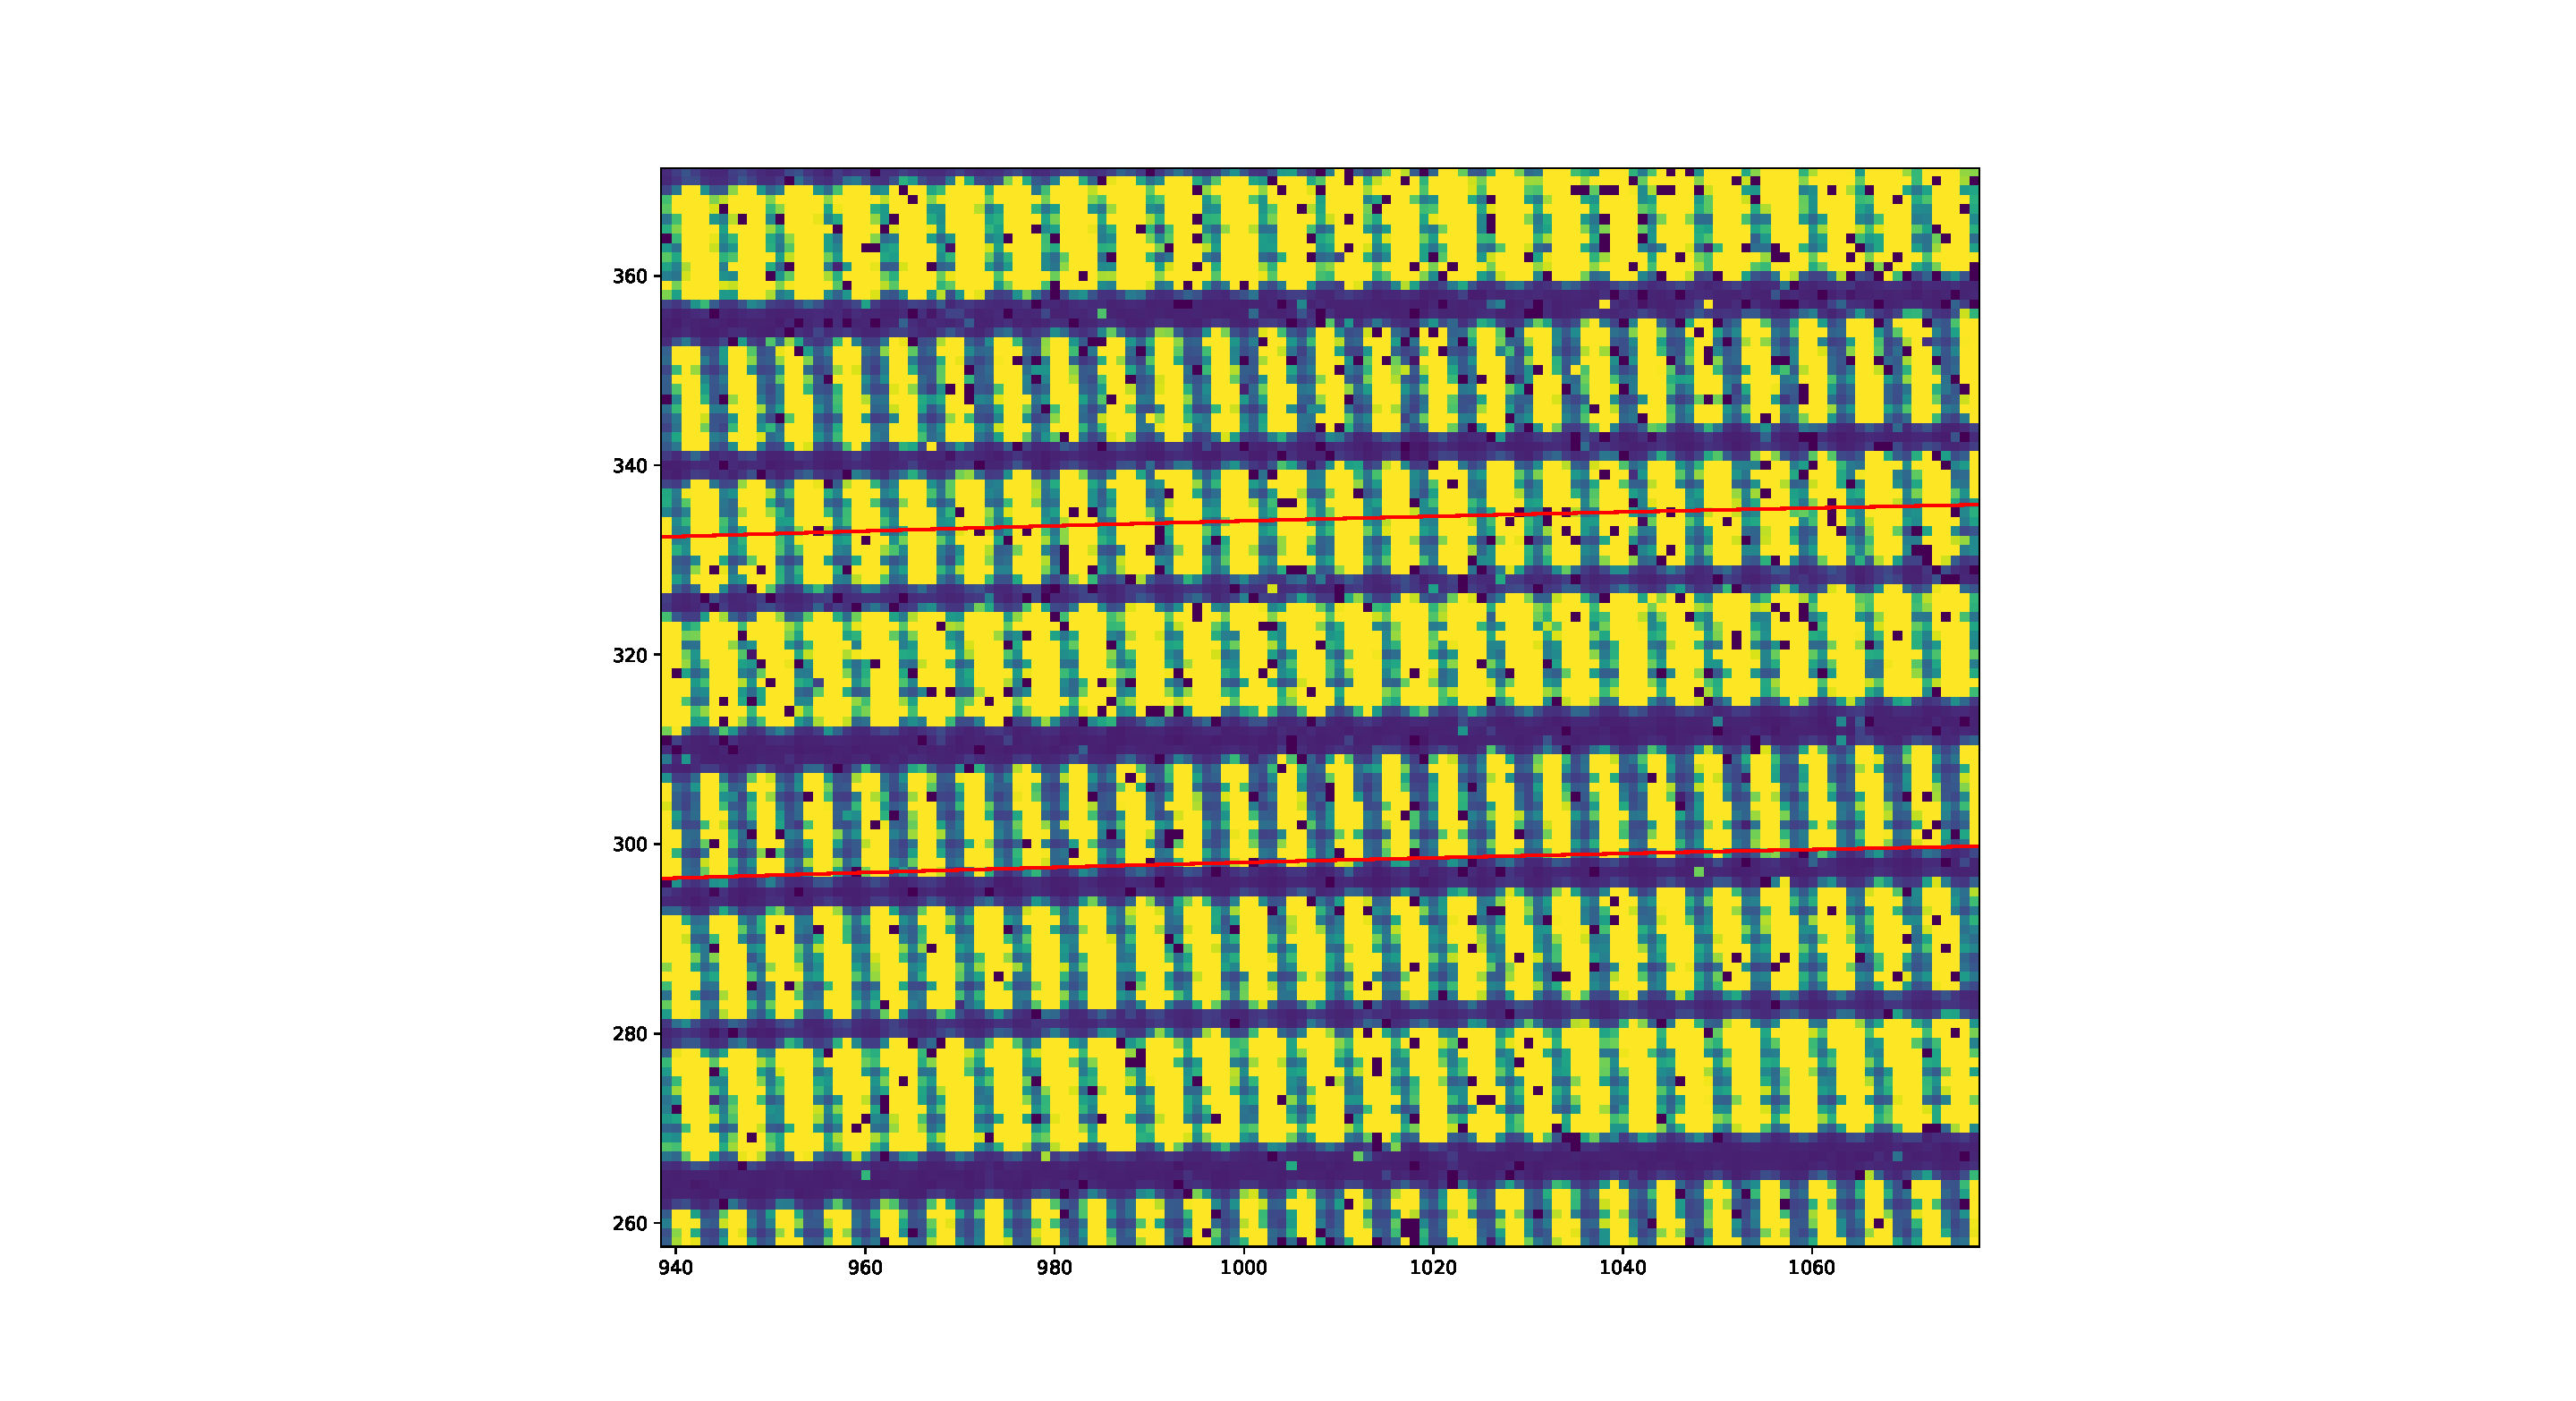
\includegraphics[width=\textwidth]{Figures/cal_SLIT_spirou_1b.pdf}
b
\end{center}
\end{minipage}%
\end{center}

\begin{center}
\begin{minipage}{.495\textwidth}
\begin{center}
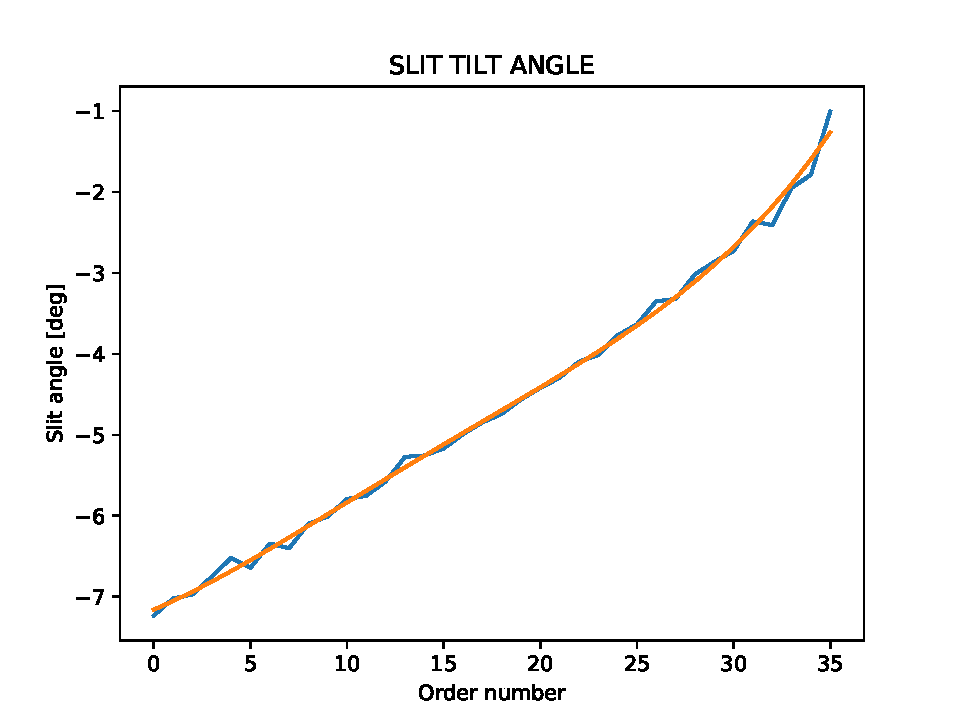
\includegraphics[width=\textwidth]{Figures/cal_SLIT_spirou_2.pdf}
c
\end{center}
\end{minipage}%
\end{center}

\caption{\textbf{(a)} The full `fp\_fp' image with one orders fit plotted. \textbf{(b)} Zoom in on a section of the `fp\_fp' image showing the tilt. \textbf{(c)} Slit angle as a function of order number with the fit to the tilt also show. \label{figure:cal_SLIT_spirou}}
\end{figure}